\documentclass{standalone}
\usepackage{tikz}
\usetikzlibrary{shapes, positioning}

\begin{document}

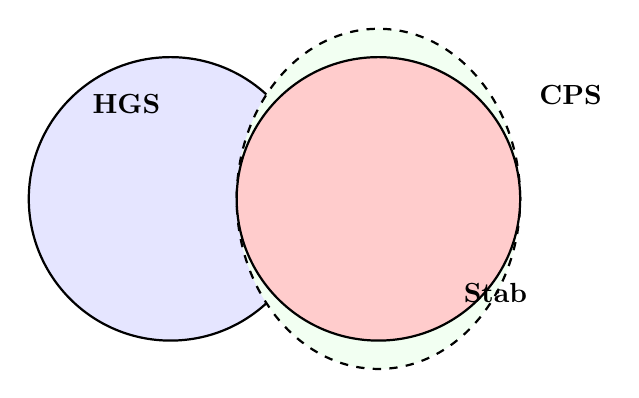
\begin{tikzpicture}[scale=1.2]
  % Define positions
  \coordinate (A) at (0,0);      % center of HGS
  \coordinate (B) at (2.2,0);    % center of Stab and CPS

  % Draw HGS (A)
  \draw[fill=blue!10, thick] (A) circle (1.5) node[left,yshift=1.2cm] {\textbf{HGS}};

  % Draw CPS (B') as an ellipse
  \draw[fill=green!5, thick, dashed] (B) ellipse [x radius=1.5, y radius=1.8];
  \node[right,yshift=1.2cm] at (3.8,0.1) {\textbf{CPS}};

  % Draw Stab (B)
  \draw[fill=red!20, thick] (B) circle (1.5);
  \node[right,yshift=-1.2cm] at (3.0,0) {\textbf{Stab}};

  % Label intersection
\end{tikzpicture}

\end{document}
